\documentclass[a4paper,12pt,oneside]{book}

% Language
\usepackage[ngerman]{babel}
\usepackage{csquotes}

% Make non-ASCII characters pastable in PDF
\usepackage[T1]{fontenc} 

% Easiest way to get outline fonts with T1 encoding
\usepackage{lmodern}

% Control design of table of contents
\usepackage{tocloft}

% Blank lines between paragraphs
\usepackage[parfill]{parskip}

% Hyperlinks
\usepackage[hidelinks]{hyperref}

% Extensions of hyperref
\usepackage{bookmark}
\usepackage{nameref}

% Images
\usepackage{graphicx}

% Bibliography
\usepackage[style=ieee,maxcitenames=2,mincitenames=1,backend=biber]{biblatex}

% Page margins
\usepackage{anysize}

% Chapter title formatting
\usepackage{titlesec}

% Remove headers and footers from empty pages
\usepackage{emptypage}

% Access to colors
\usepackage{xcolor}

% Glossaries, acronyms, and abbreviations
\usepackage[nopostdot,nogroupskip,toc,acronym,nomain]{glossaries-extra}

% Disable warnings
\usepackage{silence}

% Extension for tables
\usepackage{tabularx}

% Algorithms and pseudocode
\usepackage{algorithm}
\usepackage[noEnd=true,italicComments=false,commentColor=black]{algpseudocodex}

% Code listings
\usepackage{listings}

% Adjust captions
\usepackage{caption}

% Mathematical alphabets
\usepackage{amssymb}

% Better tables
\usepackage{booktabs}

% Add line breaks to table cells
\usepackage{makecell}

% Header and footer
\usepackage{fancyhdr}

% Appendix
\usepackage{appendix}

% Bibliography file
\addbibresource{config/literature.bib}

% Do not stretch the page contents to the bottom
\raggedbottom

% Reduce hyphenation
\tolerance=500
\emergencystretch=2em
\hyphenpenalty=500
\exhyphenpenalty=500

% Reduce widows and orphans
\widowpenalties=4 10000 10000 500 0
\clubpenalties=4 10000 10000 500 0

% Reduce page breaks in paragraphs
\interlinepenalty=500

% Margins (Left, Right, Top, Bottom)
\marginsize{25mm}{25mm}{20mm}{20mm}

% Chapter title formatting
\titleformat{\chapter}
  {\Huge\bfseries}   % format
  {\thechapter}      % label
  {10pt}             % sep
  {}                 % before-code

% Redefine command for vertical centering text in X column (tabularx)
\renewcommand\tabularxcolumn[1]{m{#1}}

% Include chapter number in algorithm numbering.
\renewcommand{\thealgorithm}{\thechapter.\arabic{algorithm}}

% Add double colon after algorithm numbering.
\captionsetup[algorithm]{labelsep=colon}

% Redefine title for list of code listings
\renewcommand{\lstlistlistingname}{List of Code Listings}

% Styling for code listings
\definecolor{stringcolor}{cmyk}{0.8, 0.0, 0.8, 0.2}
\definecolor{commentcolor}{cmyk}{0.0, 0.0, 0.0, 0.5}
\definecolor{emphcolor}{cmyk}{1.0, 0.6, 0.0, 0.2}
\definecolor{keywordcolor}{cmyk}{0.0, 0.5, 1.0, 0.2}

% Define a custom style for listings
\lstdefinestyle{custom_listing_style}{
    language=Python,
    basicstyle=\ttfamily\small,
    columns=fullflexible,
    keepspaces=true,
    frame=tb,
    rulecolor=\color{black},
    numbers=left,
    xleftmargin=2em,
    framexleftmargin=1.5em,
    numberstyle=\scriptsize,
    numbersep=8pt,
    stepnumber=1,
    breaklines=true,
    tabsize=4,
    belowcaptionskip=12pt,
    showstringspaces=false
    morekeywords={self},
    sensitive=true,
    emph={}, 
    morestring=[b]",
    morecomment=[l]{//},
    keywordstyle=\color{keywordcolor},
    stringstyle=\color{stringcolor},
    commentstyle=\color{commentcolor},
    emphstyle=\color{emphcolor},
    escapeinside={(*@}{@*)}
}
\lstset{style=custom_listing_style}

% Increase vertical padding for tables
\renewcommand{\arraystretch}{1.5}

% Header and footer
\renewcommand{\chaptermark}[1]{\markboth{#1}{}}
\fancyhead[L]{\thechapter\hspace{1.0em}\leftmark}
\fancyhead[R]{}
\fancyfoot[C]{\thepage}

% Adjust headheight for header
\setlength{\headheight}{15pt}

% Adjust algpseudocodex keywords
\algrenewcommand\algorithmicrequire{Input:}
\algrenewcommand\algorithmicensure{Output:}

% Definition of custom glossary style for list of abbreviations
\newglossarystyle{customglossarystyle}{
  \setglossarystyle{long}

  % Adjust list of abbreviations to full text width
  \renewenvironment{theglossary}
  {
    \setlength{\tabcolsep}{2pt}%
    \begin{longtable}[l]{@{}p{2.5cm}@{}p{\dimexpr\linewidth-2.5cm}@{}}
  }
  {
    \end{longtable}
  }

  % Use dotfill with same style as in table of contents
  \newcommand\Dotfill{\cftdotfill{\cftsecdotsep}}
  \renewcommand{\cftchapleader}{\cftdotfill{\cftsecdotsep}}
  \renewcommand{\glspostdescription}{\Dotfill}

  % Adjust space between title and list of abbreviations
  \setglossarypreamble[acronym]{\vspace{-0.5cm}}

  % Bold font for abbreviations
  \renewcommand{\glsnamefont}[1]{\textbf{##1}}
}

% Set up glossaries, acronyms, and abbreviations
\makeglossaries

% Set abbreviation style for acronyms
\setabbreviationstyle[acronym]{long-short}

\newacronym{dsr}{DSR}{Design Science Research}


\begin{document}

    \frontmatter
    \pagestyle{plain}
        % Uppercase Roman page numbering for front matter
        \pagenumbering{Roman}

        \begin{titlepage}
  \thispagestyle{empty}

  \makebox[\textwidth]{
      % Logo on the left:
      % 
\includegraphics[height=1.5cm]{figures/logos/hm-logo.png}
      \hfill
      % Logo on the right:
      
\includegraphics[height=1.6cm]{figures/logos/hm-logo.png}
    }

  \vspace{2cm}

  \begin{center}
    {\LARGE \textbf{Title of the Thesis} \\}
    \vspace{0.5cm}
    {\large Subtitle of the Thesis}

    \vspace{1.2cm}
    {\large \textbf{Master's Thesis} \\}
    \vspace{0.2cm}
    for the degree of Master of Science (M.Sc.)

    \vspace{1.2cm}
    Submitted to \\
    Munich University of Applied Sciences \\
    Department of Computer Science and Mathematics

    \vspace{1.2cm}
    Submitted by \\
    Max Mustermann \\
    Program of Study: Computer Science\\
    Student ID: 012345678
  \end{center}

  \vfill

\begingroup
\renewcommand{\arraystretch}{1.0}
\begin{tabular}{@{}ll@{}}
  First Examiner:  & Prof. Dr. Markus Mustermann \\
  Second Examiner: & Maria Mustermann \\
  Supervisor:    & Martin Mustermann \\
  Submission Date: & 01.01.2025 \\
\end{tabular}
\endgroup

\end{titlepage}
\addtocounter{page}{1}

        \chapter*{Sperrvermerk}
\label{confidentiality}

Die vorliegende Arbeit beinhaltet interne vertrauliche Informationen der Firma XYZ. Die Weitergabe des Inhalts der Arbeit im Gesamten oder in Teilen sowie das Anfertigen von Kopien und Abschriften sind grundsätzlich untersagt. Ausnahmen bedürfen der schriftlichen Zustimmung der Firma.

        \chapter*{Kurzfassung}
\label{abstract}

Eine kurze Zusammenfassung des Zwecks, der Methoden, der wichtigsten Ergebnisse und der Schlussfolgerungen der Arbeit.

        \chapter*{Danksagung}
\label{acknowledgments}

Ein optionaler Abschnitt, in dem Personen und Organisationen gedankt wird, die die Arbeit unterstützt oder dazu beigetragen haben.


        \clearpage
        \tableofcontents
        
        \clearpage
        \phantomsection
        \addcontentsline{toc}{chapter}{\listfigurename}
        \listoffigures
        
        % Combine List of Tables, Algorithms, and Code Listings into one page
        \clearpage
        \phantomsection
        \addcontentsline{toc}{chapter}{Tabellen-, Algorithmen- und Codeverzeichnis}
        \listoftables
        \vspace{-0.3cm}
        \begingroup
            \let\clearpage\relax
            \listofalgorithms
            \lstlistoflistings 
        \endgroup

        \printglossary[style=customglossarystyle,type=\acronymtype,title=Abkürzungsverzeichnis,toctitle=Abkürzungsverzeichnis]

    \mainmatter
    \pagestyle{fancy}

        \section{Einleitung}

Menschen, die mit ihrem IQ prahlen, sind Versager. [\cite[S. 99]{hawking_1999}]

        \chapter{Verwandte Arbeiten}
\label{chap:related-work}

\section{Tabellen}

\begin{table}[htbp]
    \centering
    \caption{Ein- und Ausschlusskriterien für das Literatur-Review.}
    \label{table:review-criteria}
    \begin{tabularx}{1.0\textwidth}{>{\raggedright\arraybackslash}X>{\raggedright\arraybackslash}X}
        \toprule
        \textbf{Einschlusskriterien}              & \textbf{Ausschlusskriterien}           \\
        \midrule
        Englische Sprache                         & Nicht-englische Sprache                \\
        Veröffentlicht 2015–2025                  & Veröffentlicht vor 2015                \\
        Peer-reviewed                             & Nicht peer-reviewed                    \\
        Liefert Methode und empirische Ergebnisse & Irrelevantes Fachgebiet oder Off-Topic \\
        \bottomrule
    \end{tabularx}
\end{table}

Man kann Tabellen erstellen und sie wie folgt referenzieren: Tabelle~\ref{table:review-criteria} zeigt die Ein- und Ausschlusskriterien für das Literatur-Review.

\section{Zitate}

Quellen können in Klammern wie folgt zitiert werden: Designmuster erleichtern die Wiederverwendung erfolgreicher Entwürfe und Architekturen \autocite{gamma1994design}.

Quellen können auch direkt im Text zitiert werden: \textcite{gamma1994design} bietet einen umfassenden Überblick über Designmuster.

        \chapter{Methodik}
\label{chap:methodology}

\section{Abkürzungen}

Man kann Abkürzungen definieren und wie folgt darauf verweisen: Die \gls{dsr}-Methodik wird häufig in der Forschung zu Informationssystemen verwendet. Der \gls{dsr}-Ansatz betont die Erstellung und Evaluierung von Artefakten zur Lösung identifizierter Probleme.

\section{Abbildungen}

\begin{figure}[htbp!]
    \centering
    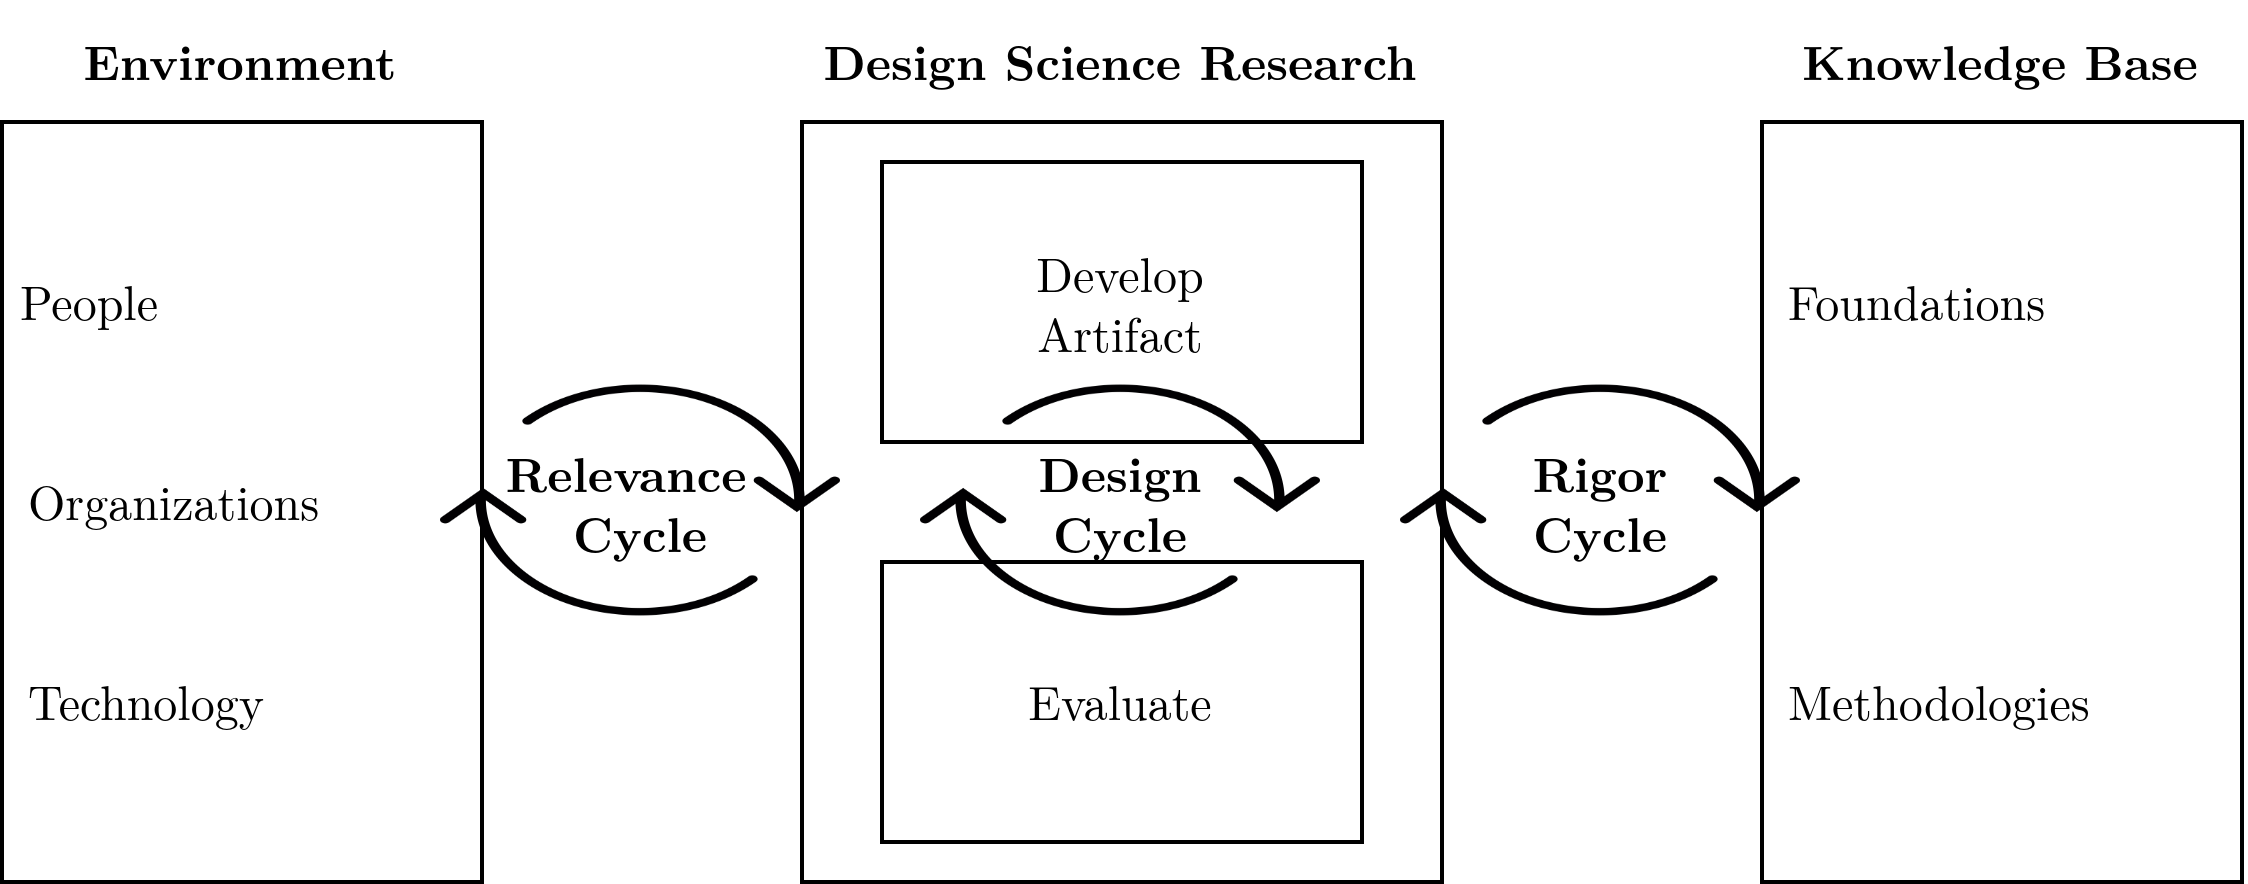
\includegraphics[width=0.9\textwidth]{figures/design-science-generic.png}
    \caption[DSR-Ansatz mit Relevanz-, Rigorositäts- und Design-Zyklus.]{DSR-Ansatz mit Relevanz-, Rigorositäts- und Design-Zyklus. Adaptiert aus~\textcite{hevner2004design}.}
    \label{fig:design-science-generic}
\end{figure}

Man kann Abbildungen einfügen und wie folgt darauf verweisen: Abbildung~\ref{fig:design-science-generic} zeigt den \gls{dsr}-Ansatz mit Relevanz-, Rigorositäts- und Design-Zyklus.

        \chapter{Implementation}
\label{chap:implementation}

\section{Formulas}

You can include formulas like this: The file processing problem can be modeled as follows. A file $F$ of size $S$ bytes split into chunks of size at most $c$ is:
\[ F = \langle B_1, B_2, \ldots, B_m \rangle, \qquad m = \left\lceil \frac{S}{c} \right\rceil \]

\section{Algorithms}

You can describe algorithms using pseudocode like this:

\begin{algorithm}[htbp]
    \caption{Chunk-based file processing with hashing.}
    \label{algo:filehash}
    \begin{algorithmic}[1]
        \Require File $F$, chunk size $c$
        \Ensure Record $\langle size, chunk\_count, sha256 \rangle$

        \State $h \gets \textsc{InitSHA256}()$ \Comment{Initialize digest.}
        \State $size \gets \textsc{Length}(F)$
        \State $chunk\_count \gets 0$
        \Statex

        \ForAll{$chunk \in \textsc{Read}(F, c)$}
        \State $\textsc{Update}(h, chunk)$
        \State $chunk\_count \gets chunk\_count + 1$
        \EndFor
        \Statex

        \State $sha256 \gets \textsc{Finalize}(h)$
        \State \Return $\langle size, chunk\_count, sha256 \rangle$
    \end{algorithmic}
\end{algorithm}

You can refer to algorithms like this: Algorithm~\ref{algo:filehash} describes a chunk-based file processing algorithm.

\section{Lists and Enumerations}

You can create lists and enumerations like this:

\begin{enumerate}
    \item Initialize SHA-256 digest and read the file size.
    \item Stream the file in chunks of at most $c$ bytes.
    \item For each chunk, update the digest and increment the chunk counter.
    \item Finalize the digest to obtain the hash.
    \item Return $\langle size,\ chunk\_count,\ sha256 \rangle$.
\end{enumerate}

\subsection{Code Listings}

You can include source code listings, for example Python code, like this:

\begin{lstlisting}[float=htb, caption={Source code of the file processing algorithm.}, label={lst:filehash}]
import hashlib
from pathlib import Path

def process_file(path: str, chunk_size: int = 1 << 20):
    p = Path(path)
    h = hashlib.sha256()
    with p.open("rb") as f:
        while True:
            b = f.read(chunk_size)
            if not b:
                break
            h.update(b)
    return {
        "file": p.name,
        "size_bytes": p.stat().st_size,
        "sha256": h.hexdigest()
    }

if __name__ == "__main__":
    print(process_file("example.dat"))
\end{lstlisting}

        \chapter{Results}
\label{chap:results}

\section{Graphs}

This is a graph which was created using Python (Jupyter Notebook) to match the style of the document.

\begin{figure}[htbp]
    \centering
    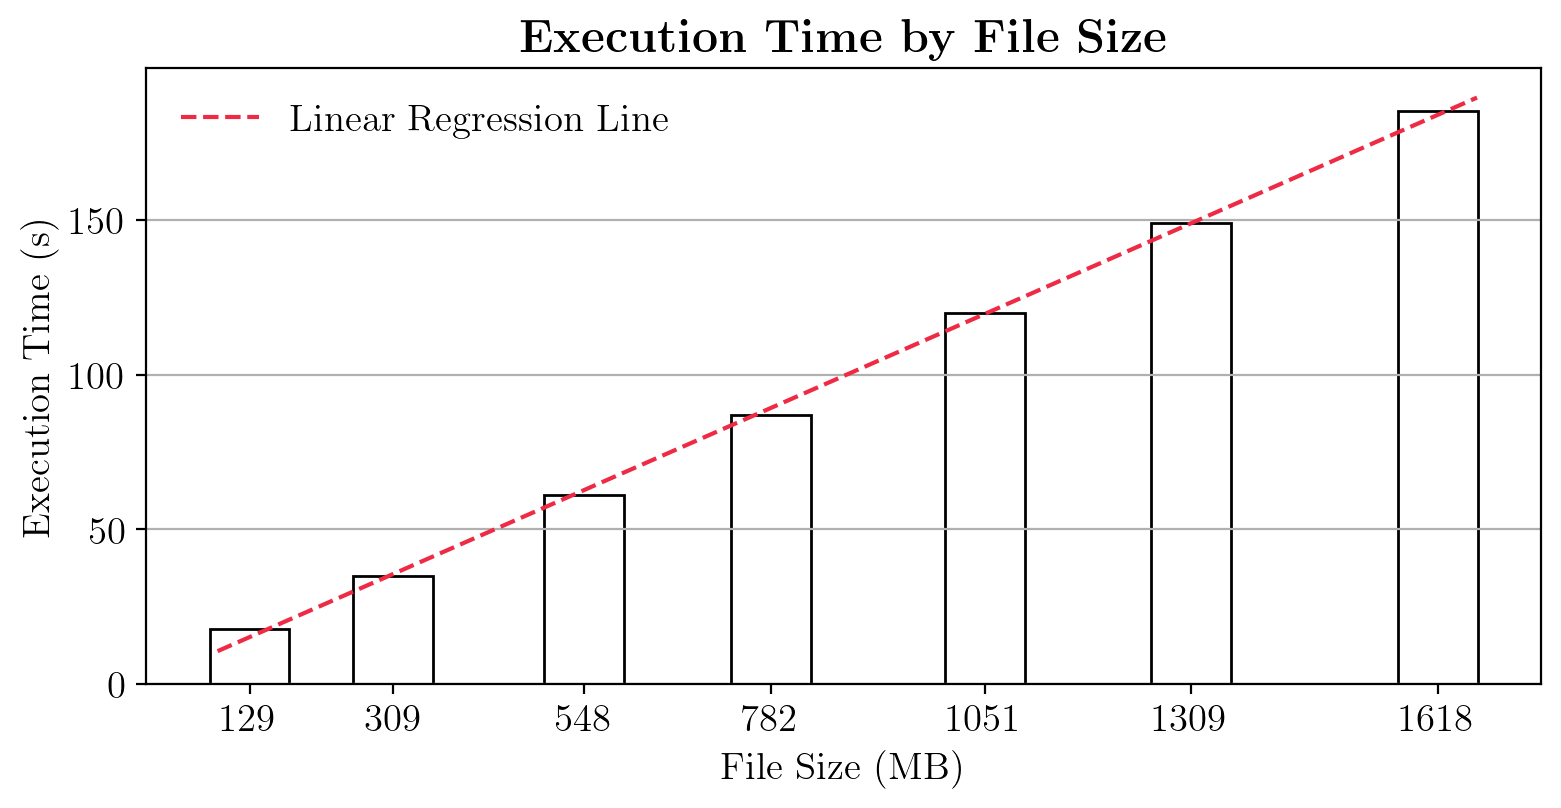
\includegraphics[width=0.9\textwidth]{figures/execution-time.png}
    \caption{Execution time by trace file size of the framework.}
    \label{fig:execution-time}
\end{figure}

        \chapter{Fazit}
\label{chap:conclusion}

\section{Gantt-Diagramm}

Dies ist ein Gantt-Diagramm, das mit draw.io erstellt wurde, um den Stil des Dokuments beizubehalten.

\begin{figure}[htbp]
    \centering
    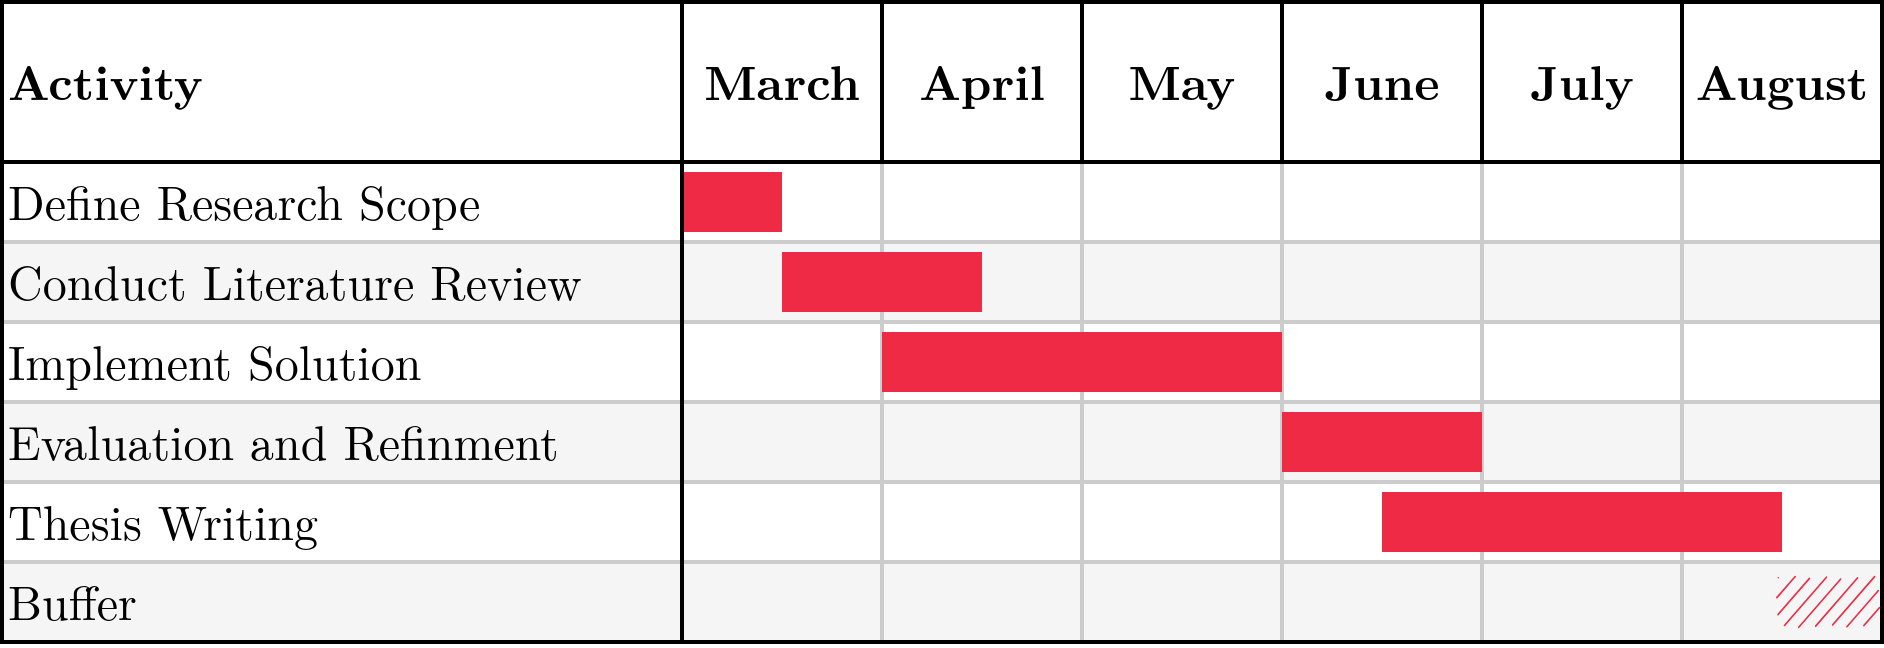
\includegraphics[width=0.9\textwidth]{figures/gantt-chart.png}
    \caption{Gantt-Diagramm des Projektzeitplans.}
    \label{fig:gantt-chart}
\end{figure}


    \appendix
    \pagestyle{plain}

        \printbibliography[heading=bibintoc]
        \addcontentsline{toc}{chapter}{Ehrenwörtliche Erklärung}
        \chapter*{Ehrenwörtliche Erklärung}
\label{declaration}

Hiermit erkläre ich, dass ich die vorliegende Masterarbeit selbständig verfasst, noch nicht anderweitig für Prüfungszwecke vorgelegt, keine anderen als die angegebenen Quellen oder Hilfsmittel benützt sowie wörtliche und sinngemäße Zitate als solche gekennzeichnet habe.

\vspace{1.5cm}
\begin{tabular*}{\textwidth}{%
  @{\extracolsep{\fill}}
  w{l}{5.5cm}
  c
  w{l}{5.5cm}
  @{}
}
München, 01.01.2025 && 
\includegraphics[height=1.3cm]{figures/logos/signature.png} \\
\cmidrule(r){1-1}\cmidrule(l){3-3}
Ort, Datum && Unterschrift
\end{tabular*}
        
        \begin{appendices}

    \chapter{Anhang}
    \label{appendix}

    \section{Zusätzliches Material}

\end{appendices}


\end{document}
